\section{Interviews mit anderen Agenturen}
Da allink nicht die erste Agentur ist, die sich den Herausforderungen der
Organisation und des Projektmanagement stellt, macht es Sinn sich in der Branche
umzusehen und ähnliche Agenturen zu befragen. Der Studierende erhofft sich aus
den Resultaten Hinweise und Tipps bezüglich Projektmanagement und mögliche
Tools die unterstützend eingesetzt werden können.

Als Interviewpartner werden möglichst ähnliche Agenturen wie die allink gesucht.
Optimal sind Agenturen, die die Herausforderung des Wachstums schon meistern
konnten. Der Studierende fragt in Zürich ein paar vergleichbare Agenturen an.

\subsection{Fragekatalog}
Der in der Tabelle \ref{tab:fragekatalog} dargestellte Fragekatalog wurde für 
das Interview mit einer anderen Unternehmung aufgebaut. Die einzelnen Themenblöcke 
und die Zusammenstellung der Fragen wurden gezielt auf die Struktur der bestehenden 
IST-Analyse der allink zusammengestellt um einen möglichst guten Vergleich darstellen 
zu können.

\newcounter{qcounter}
\begin{longtable}{lp{14cm}}
    \toprule \textbf{Nr.} & \textbf{Frage} \\
    \midrule & \textbf{Allgemeine Fragen} \\
    \midrule \addtocounter{qcounter}{1}\arabic{qcounter} & Wer ist mein Interviewpartner? \\
    \midrule \addtocounter{qcounter}{1}\arabic{qcounter} & Was ist die Funktion meines Interviewpartners? \\
    \midrule \addtocounter{qcounter}{1}\arabic{qcounter} & Was sind die Aufgaben meines Interviewpartners? \\
    \midrule & \textbf{Unternehmen} \\
    \midrule \addtocounter{qcounter}{1}\arabic{qcounter} & Wann wurde das Unternehmen gegründet? \\
    \midrule \addtocounter{qcounter}{1}\arabic{qcounter} & Wie viele Partner mit Mitspracherecht existieren? \\
    \midrule \addtocounter{qcounter}{1}\arabic{qcounter} & Wie ist das Organigramm des Unternehmens aufgebaut? \\
    \midrule \addtocounter{qcounter}{1}\arabic{qcounter} & Wie viele Vollzeitangstellte werden beschäftigt? \\
    \midrule \addtocounter{qcounter}{1}\arabic{qcounter} & Sind Praktikanten angestellt? \\
    \midrule \addtocounter{qcounter}{1}\arabic{qcounter} & Bietet das Unternehmen Lehrstellen an? \\
    \midrule & \textbf{Kunden} \\
    \midrule \addtocounter{qcounter}{1}\arabic{qcounter} & Wie viele Kunden sind Kleinstunternehmen? \\
    \midrule \addtocounter{qcounter}{1}\arabic{qcounter} & Wie viele Kunden sind kleine Unternehmen? \\
    \midrule \addtocounter{qcounter}{1}\arabic{qcounter} & Wie viele Kunden sind mittlere Unternehmen? \\
    \midrule \addtocounter{qcounter}{1}\arabic{qcounter} & Wie viele Kunden sind grosse Unternehmen? \\
    \midrule & \textbf{Projektablauf} \\
    \midrule \addtocounter{qcounter}{1}\arabic{qcounter} & Wie viele Projekte werden akquiriert? \\
    \midrule \addtocounter{qcounter}{1}\arabic{qcounter} & Wie viele Projekte entstehen durch direkte Anfragen? \\
    \midrule \addtocounter{qcounter}{1}\arabic{qcounter} & Wie werden die Aufwände eines potenziellen Projektes geschätzt? \\
    \midrule \addtocounter{qcounter}{1}\arabic{qcounter} & Wie wird auf Änderungen während des Projektes reagiert? \\
    \midrule \addtocounter{qcounter}{1}\arabic{qcounter} & Kommt es vor, dass Projekte während der Durchführung abgebrochen werden? \\
    \midrule \addtocounter{qcounter}{1}\arabic{qcounter} & Von wem werden die Arbeitspakete zusammengestellt? \\
    \midrule \addtocounter{qcounter}{1}\arabic{qcounter} & Wie werden die Arbeitspakete verteilt? \\
    \midrule \addtocounter{qcounter}{1}\arabic{qcounter} & Wie werden die Aufwände rapportiert? \\
    \midrule \addtocounter{qcounter}{1}\arabic{qcounter} & Wer kommuniziert direkt mit einem Kunden? \\
    \midrule \addtocounter{qcounter}{1}\arabic{qcounter} & Wie wird das Feedback eines Kunden verarbeitet? \\
    \midrule \addtocounter{qcounter}{1}\arabic{qcounter} & Wie wird mit zusätzlich zu verrechnenden Anforderungen verfahren? \\
    \midrule \addtocounter{qcounter}{1}\arabic{qcounter} & Wie werden die Projektdaten archiviert? \\
    \midrule & \textbf{Verwendete Software} \\
    \midrule \addtocounter{qcounter}{1}\arabic{qcounter} & Auf welches Betriebssystem setzt das Unternehmen? \\
    \midrule \addtocounter{qcounter}{1}\arabic{qcounter} & Welche Office Suite setzt das Unternehmen ein? \\
    \midrule \addtocounter{qcounter}{1}\arabic{qcounter} & Was für Projektmanagement-Software wird verwendet? \\
    \midrule & \textbf{Stärken und Schwächen} \\
    \midrule \addtocounter{qcounter}{1}\arabic{qcounter} & Wo liegen die Stärken des Unternehmens? \\
    \midrule \addtocounter{qcounter}{1}\arabic{qcounter} & Wo sieht das Unternehmen ihre Chancen? \\
    \midrule \addtocounter{qcounter}{1}\arabic{qcounter} & Wo liegen die Schwächen des Unternehmens? \\
    \midrule \addtocounter{qcounter}{1}\arabic{qcounter} & Mit was für Risiken sieht sich das Unternehmen konfrontiert? \\
    \bottomrule
    \caption[Fragekatalog zur Marktanalyse]{Fragekatalog zur Marktanalyse\footnotemark}
    \label{tab:fragekatalog}
\end{longtable}
\footnotetext{Eigene Darstellung}

Der erstellte Fragenkatalog dient als Leitfaden im Interview. Die Antworten
werden entgegengenommen, diskutiert und anschliessend in beschreibender Form
dokumentiert. Die verweisenden Fragen werden in Klammern an der dazugehörigen
Textstelle angegeben. Falls gewissen Fragen nicht beantwortet wurden, wird dies 
erwähnt und begründet.

\subsection{Panter IIc}
Das Unternehmen Panter IIc mit Sitz in Zürich hat sich freundlicherweise dazu
bereiterklärt mit dem Studierenden ein Interview durchzuführen. Der Interview
Partner ist Syrus Mozafar. Er ist Teilhaber der Panter IIc und Mitglied der
Geschäftsleitung (\textbf{1}).

Er ist laut eigenen Angaben auch für das Projektmanagement zuständig (\textbf{2})
und oft selbst Projektleiter. Sein Aufgabenbereich liegt speziell in der 
Projektplanung, Konsolidierung der Ressourcenplanung und das Auszahlen von
Löhnen in der Buchhaltung (\textbf{3}).

\subsubsection{Unternehmen}
Das Unternehmen ist im Jahre 2005 als GmbH gegründet worden. Die Rechtsform
ist bis heute erhalten geblieben (\textbf{4}). Es existieren fünf Teilhaber,
jedoch kann in ihrer Firmenkultur jeder Mitarbeiter bei grösseren Entscheidungen
des Unternehmens mitentscheiden (\textbf{5}).

Es existiert zur Zeit kein richtiges Organigramm, die Struktur ist flach
und jeder Mitarbeiter hat gewisse Kompetenzen und Aufgaben (\textbf{6}). 
Insgesamt hat Panter zwölf Mitarbeiter und zusätzliche sechs Mitarbeiter im
Personalverleih. Die Anstellungspensum variiert zwischen 20\% bis 80\% (\textbf{7}).
Zur Zeit wird ein Praktikant, jedoch noch keine Lehrlinge beschäftigt und die Geschäftsleitung
wird dies zu diesem Zeitpunkt nicht ändern, da sie darin eher einen Mehraufwand
als Nutzen sehen (\textbf{8} und \textbf{9}).

\subsubsection{Kunden}
Panter verfügt über einen relativ grossen Kundenstamm. Die Verteilung
der Unternehmensgrössen der Kunden unterteilen sich in ca. 40\% Kleinstunternehmen,
20\% kleine Unternehmen, 10\% mittlere Unternehmen und 30\% grosse
Unternehmen (\textbf{10} bis \textbf{13}).

\subsubsection{Projektablauf}
Bei Panter werden ca. 20\% der Projekte selbst akquiriert (\textbf{14}) und ca.
80\% entstehen durch direkte Anfragen oder Folgeaufträge (\textbf{15}). Kleinere
Projekte mit einem Umsatzvolumen bis 20'000 CHF werden nur grob im Alleingang
des Projektleiters geschätzt. Bei grösseren Projekten werden auf Grund der
Technologiewahl Experten innerhalb von Panter oder ausserhalb herbeigezogen
um eine möglichst genaue Schätzung abgeben zu können (\textbf{16}). Sie verwenden
dazu keine speziellen Verfahrenstechniken und setzen überwiegend die Software
Microsoft Excel ein. Bei grösseren Änderungen während eines Projektes wird
erneut eine Schätzung vorgenommen und dem Kunden die zusätzlichen Aufwände
offeriert (\textbf{17}). Es wird von Fall zu Fall entschieden ob eine Änderung 
zusätzlich verrechnet oder dem Kunden ``geschenkt'' wird (\textbf{24}). Bis zu 
diesem Zeitpunkt kam es erst einmal zu einem vollständigen Abbruch eines Projektes 
während dessen Durchführung (\textbf{18}).

Die Arbeitspakete werden überwiegend während der Erstellung der Schätzung und 
der Offerte vom Projektleiter und den Experten zusammengestellt (\textbf{19}).
Dabei ist im Normalfall immer auch eine Person der Geschäftsleitung vertreten.
Die Arbeitspakete werden dann auch gleich von dieser Gruppe an die für das 
Projekt eingeplanten Ressourcen verteilt (\textbf{20}).

Die Aufwände werden von den Mitarbeitern sehr exakt rapportiert (\textbf{21}),
da die Lohnsummen der einzelnen Mitarbeiter von den Anzahl geleisteten Stunden
abhängt. Es existieren somit keine Fixlöhne bei Panter.

Die Kommunikation mit dem Kunden erfolgt im Normalfall über den Projektleiter.
Es kommt aber auch vor, dass ein Mitarbeiter direkt bei einem Kunden zusätzliche
Informationen einfordert (\textbf{22}). Es existieren keine fixen Regeln dazu.
Das Feedback des Kunden wird im Unternehmens Wiki eingetragen. Da die zerstreute
Verteilung der Projektdaten in der Vergangenheit schon öfters bemängelt wurde, 
baut Panter zu diesem Zeitpunkt eine Struktur für ein Projektarchiv auf. Sie
verwenden zudem ein allgemeines E-Mail Konto um projektspezifische E-Mails
zentral und für alle Mitarbeiter zugänglich abzulegen (\textbf{23} und \textbf{25}).

\subsubsection{Verwendete Software}
Das Unternehmen setzt auf kein spezifisches Betriebssystem. Jeder Mitarbeiter
hat sein eigenes Gerät mit seinem präferierten System installiert. Einzig für
die unternehmenseigenen Server wird das Betriebssystem Debian\footnote{Debian 
ist ein frei verfügbares Betriebssystem, \url{http://www.debian.org/}} 
vorausgesetzt (\textbf{26}).

Also Office Suite setzt Panter auf die Open-Source
Lösung OpenOffice\footnote{OpenOffice ist eine frei verfügbare Office Suite, 
\url{http://de.openoffice.org/}}. Zusätzlich, um Interoperabilitätsprobleme
mit Kunden zu vermeiden, hat Panter eine Arbeitsstation mit Microsoft Windows
und Microsoft Office ausgerüstet (\textbf{27}).

Panter setzt überwiegend auf die Projektmanagement Software RedMine\footnote{RedMine
ist eine Webapplikation für Projektmanagement, \url{http://www.redmine.org/}},
wobei sie diese nicht vollständig sondern nur Teile davon nutzen (\textbf{28}). 
Das unternehmenseigene Wiki und diverse Exceldokumente unterstützen die in RedMine
verwalteten Projekte. 

\subsubsection{Stärken und Schwächen}
Die Stärken sieht Panter zur Zeit überwiegend in ihrer Grösse und der flachen
Struktur. Mit dieser können ihre Projekte zur Zeit sehr erfolgreich durchgeführt 
werden. Auch sehen sie das Mitspracherecht aller Mitarbeiter als grossen Vorteil.
Zusätzlich sei auch die verwendete und moderne Technologie bis jetzt immer
ein grosser positiver Faktor gewesen (\textbf{29}).

Chancen sehen sie ebenfalls im Wachstum der Agentur und allgemein könnten
sie effizienter werden. Die Schätzverfahren können noch verbessert werden und
in Zukunft möchten sie mehr auf Leistung und nicht pauschal verrechnen können (\textbf{30}).

Die Schwächen liegen hingegen bei den nicht vollständig geregelten 
Verantwortungsbereichen und dass sie keine Cashcow\footnote{Als Cashcow bezeichnet
man in der Betriebswirtschaftslehre ein Produkt oder einen Kunden, mit dem man
laufend hohe Gewinne erwirtschaften kann.} besitzen (\textbf{31}).

Als Risiko sehen sie die schwankende Liquiditätsplanung, die nur auf zwei Monate 
hinaus garantiert werden kann. Zusätzlich fürchten sie eine negative Veränderung 
der Firmenkultur bei einem weiteren Wachstum (\textbf{32}).

\subsection{FEINHEIT GmbH}
Das Unternehmen FEINHEIT GmbH mit Sitz in Zürich hat sich freundlicherweise
ebenfalls dazu bereiterklärt mit dem Studierenden ein Interview zum Branchenvergleich
durchzuführen. Der Interview Partner ist Matthias Kestenholz. Er ist einer der
fünf Gründer der FEINHEIT (\textbf{1}). Seine Funktion lässt sich als CTO\footnote{Der Chief Technical Officer (CTO) ist
für die technische Entwicklung und Forschung innerhalb eines Unternehmens
verantwortlich.} am Besten umschreiben (\textbf{2}). Er leitet zu 20\% die
technische Entwicklung und entwickelt selber noch 80\% seiner Arbeitszeit. Er
ist zudem zuständig für den Aufbau der Qualitätskontrolle und hat das letzte
Wort bei einer Neuanstellung in der Informatik (\textbf{3}).

\subsubsection{Unternehmen}
Das Unternehmen ist im Jahre 2005 als GmbH gegründet worden. Die Rechtsform
ist bis heute erhalten geblieben (\textbf{4}). Die FEINHEIT hat sich vor ca. 
einem halben Jahr viele Gedanken zur Organisation ihres Unternehmens gemacht 
und eine klare Struktur erstellt. Das aktuelle Organigramm ist in der Grafik 
\ref{pic:organigramm_feinheit} abgebildet.

\begin{figure}[h!]
\begin{center}
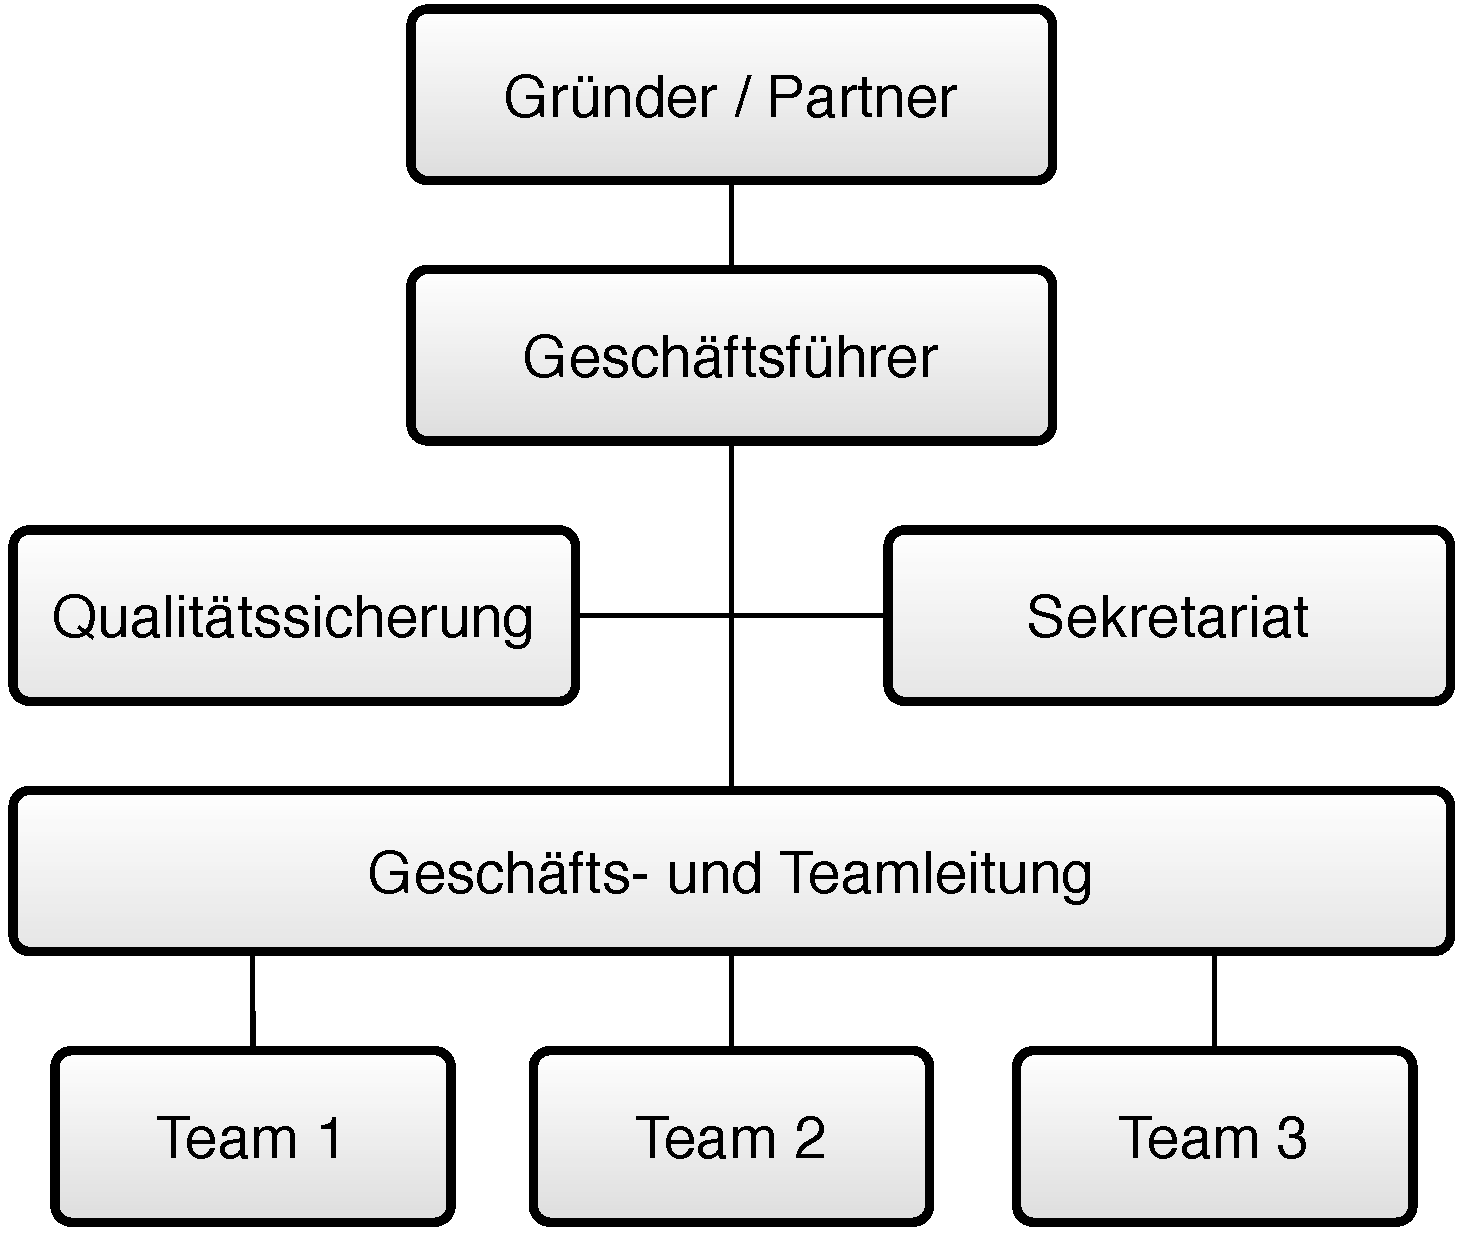
\includegraphics[width=0.39\textwidth,angle=0]{./bilder/analyse/organigramm_feinheit.pdf}
\caption[Organigramm der FEINHEIT GmbH]{Organigramm der FEINHEIT GmbH\footnotemark}
\label{pic:organigramm_feinheit}
\end{center}
\end{figure}
\footnotetext{Eigene Darstellung nach der Beschreibung von Matthias Kestenholz.}

\clearpage

Es existieren fünf Partner bzw. Gründer (\textbf{5}) und ein Geschäftsführer,
der gleichzeitig auch ein Partner ist. Die Stabsstellen Qualitätssicherung setzten
sich aus zwei und das Sekretariat aus einer Person zusammen. In der Geschäfts-
bzw. Teamleitung existieren pro Team ein bis zwei Teamleiter und die Teams
setzen sich aus vier bis sieben Mitarbeitern zusammen (\textbf{6}).

Insgesamt beschäftigt die FEINHEIT zwanzig Mitarbeiter. Das Anstellungspensum
variiert zwischen 60\% und 100\% (\textbf{7}). Darunter sind zwei Praktikanten (\textbf{8})
jedoch noch keine Lehrlinge (\textbf{9}) beschäftigt. Es wird aber angestrebt
bis gleichzeitig drei Praktikanten und in Zukunft auch Lehrlinge zu beschäftigen.

\subsubsection{Kunden}
Die FEINHEIT verfügt über einen realtiv grossen Kundenstamm. Die Verteilung der
Unternehmensgrössen der Kunden unterteilen sich in ca. 30\% Kleinstunternehmen,
30\% kleine Unternehmen, 10\% mittlere Unternehmen und 30\% grosse Unternehmen 
(\textbf{10} bis \textbf{13}).

\subsubsection{Projektablauf}
Bei der FEINHEIT werden ca. 20\% bis 30\% der Projekte selbst akquiriert (\textbf{14})
und ca. 70\% bis 80\% entstehen durch direkte Anfragen oder Folgeaufträge (\textbf{15}).
Die Aufwände eines potenziellen Projektes werden von einem Teamleiter, der auch
gleich die Aufgabe des Projektleiters einnimmt, zusammen mit dessen Team geschätzt.
Die Schätzungen basieren überwiegend auf Referenzprojekten und Erfahrungswerten (\textbf{16}).
Bei Veränderungen während eines Projektes wird in den meisten Fällen eine Nachofferte
erstellt. Es kommt auch vor, dass keine Nachofferte erstellt werden kann, wenn 
sich die erste Offerte von den neuen Aufwänden nicht klar abgegrenzt hat (\textbf{17} und \textbf{24}).
Selten wurde ein Projekt während der Durchführung abgebrochen, wenn, dann bis
jetzt immer von Seiten der Kunden (\textbf{18}).

Die Arbeitspakete werden vom Teamleiter zusammen mit dem Team erarbeitet (\textbf{19})
und auch gleich auf die einzelnen Mitarbeiter im selben Team verteilt (\textbf{20}).
Wenn das Team nicht über genügend Ressourcen für das Projekt verfügt, kann der
Teamleiter sich mit den anderen Teamleitern absprechen und temporär eine freie
Ressource eines anderen Teams in das Projekt miteinbeziehen.

Die Aufwände werden von den Mitarbeitern sehr exakt auf 0.1 Stunden genau 
rapportiert (\textbf{21}). Diese dienen zusätzlich zur Kontrolle der Arbeitszeiten
der einzelnen Mitarbeitern. Es müssen pro Tag abzüglich der gesetzlich 
vorgeschriebenen Pausen im Schnitt 7.9 Stunden rapportiert werden. Die Teams
innerhalb des Unternehmens funktionieren als Profitcenters\footnote{Als Profitcenter
wird ein organisatorischer Teil eines Unternehmens, für den separat dessen Erfolg
gemessen wird, bezeichnet.} und der Teamleiter ist für die Kontrolle und Führung 
seines Teams zuständig.

Die Kommunikation mit dem Kunden erfolgt im Normalfall über den Teamleiter. Es
kann aber auch vorkommen, dass ein Mitarbeiter direkt bei einem Kunden zusätzliche
Informationen einfordert (\textbf{22}). Der Teamleiter hat die Aufgabe den 
Überblick über das Projekt zu behalten (\textbf{23}). Die Daten aller laufenden
und archivierten Projekte werden auf einem zentralen Server gespeichert und alle
Mitarbeiter greifen direkt auf die selben Daten zu (\textbf{25}). Um dies zu 
ermöglichen musste ab einer gewissen Grösse ein stärkerer Server und ein 
leistungsstarkes Netzwerk installiert werden.

\subsubsection{Verwendete Software}
Das Unternehmen setzt auf die Betriebssysteme MacOS X und Linux. Wobei ca.
95\% der Arbeitsstationen MacOS X installiert haben. Auf einer Handvoll 
Arbeitsstationen ist zudem VirtualBox\footnote{VirtualBox ist eine frei verfügbare
Virtualisierungssoftware von Oracle.} mit einer Windows Installation eingerichtet (\textbf{26}).
Dies überwiegend zu Testzwecken und zur Qualitätskontrolle.

Die FEINHEIT setzt überwiegend auf die Office Suite von Apple. Verwendet wird
jedoch auch OpenOffice. Ganz selten Microsoft Office über VirtualBox (\textbf{27}).
Zur Erstellung von Präsentation wird seit neustem auch Landslide\footnote{Landslide
ist ein OpenSource Lösung um Präsentationen mit der HTML5 Technik zu erstellen.} 
eingesetzt.

Das am häufigsten eingesetzte Hilfsmittel zur Unterstützung des Projektmanagement
ist das Whiteboard\footnote{Whiteboard ist keine Software sondern eine einfache
weisse Tafel auf der mit Kreide oder Stiften geschrieben werden kann.}. Die 
wichtigste Software ist jedoch die Eigenentwicklung Metronom\footnote{Metronom 
ist eine kostenpflichtige und webbasierte Firmensoftware. \url{http://fineware.ch/}}, worüber die ganze
Projekt-, Ressourcen-, Lohn- und Arbeitszeitverwaltung läuft (\textbf{28}). Teilweise wird
noch Trac\footnote{Trac ist eine frei verfügbare und webbasierte 
Projektmanamgement-Software speziell für Softwareprojekte.} eingesetzt, jedoch 
werden diese Projekte vor zu von Metronom abgelöst.

\subsubsection{Stärken und Schwächen}
Die Stärken sieht die FEINHEIT zur Zeit in ihrem ``kreativen Chaos'' und ihrem
Team. Sie arbeiten nach dem Motto ``We can do it!'' und fürchten sich nicht 
vor neuen Herausforderungen (\textbf{29}).

Ihre Chancen sehen sie in der Erschaffung der Möglichkeit sogenannte ``Robin Hood''-Projekte,
also Non-Profit Projekte, durchführen zu können. Zudem möchten sie stets ein
gutes Lernumfeld für alle Mitarbeitenden bleiben (\textbf{30}).

Gleichzeitig sehen Sie die Stärke des Chaos auch als ihre grösste Schwäche und 
zwar überwiegend in der fehlenden Konsolidierung innerhalb des Unternehmens. 
Dem wurde aber seit der Umstrukturierung vor einem halben Jahr stark entgegen
gewirkt und hat sich bereits verbessert (\textbf{31}).

Das grösste Risiko sehen sie in einem weiteren Wachstum und dem möglichen 
Verlust des Familiengefühls innerhalb des Unternehmens (\textbf{32}).

\section{Zwischenfazit}
Der Branchenvergleich mit den anderen Unternehmen mit ähnlicher Grösse und
Dienstleistungen war sehr interessant und aufschlussreich. Bei der Panter IIc
ist vor allem der Ansatz, dass alle Mitarbeiter bei Entscheidungen des 
Unternehmens mitreden dürfen sehr interessant. Sie befinden sich jedoch noch
in einer Unternehmensgrösse, bei der sich viele Herausforderungen, denen die allink 
gegenüber steht, noch nicht ergeben haben. Auch hat allink gewisse Herausforderungen,
wie zum Beispiel die Beschäftigung von Praktikanten und Lehrlingen, schon gemeistert.

Die FEINHEIT GmbH bietet da mehr interessante Ansätze und Lösungen. Vor allem
die Struktur scheint gut zu skalieren und ermöglicht anscheinend ein gesundes Wachstum.
Auch ist die Erschaffung von Stellen wie die Qualitätssicherung und das Sekretariat,
die keinen direkten Profit für das Unternehmen generieren, ein Indiz für ein
gutes Vorgehen und besseres Projektmanagement. Laut eigenen Aussagen machen sie
überwiegend den konsequenten Einsatz des Projektmanagement Tools Metronom dafür
verantwortlich. Dies ist jedoch nur ein Mittel zum Zweck und kann auf
diverse Arten umgesetzt werden.

Bei der Erarbeitung des Lösungsansatzes des neuen Projektmanagements für allink 
im Kapitel \ref{chap:loesungsansatz} werden diese Erkenntnisse einfliessen.
